\documentclass[tikz]{standalone}
\usepackage{amsmath}
\definecolor{bgcol}{HTML}{171D2B}
\definecolor{acc}{HTML}{F7B538}
\begin{document}
\pagecolor{bgcol}
\definecolor{tx}{HTML}{FFFFFF}
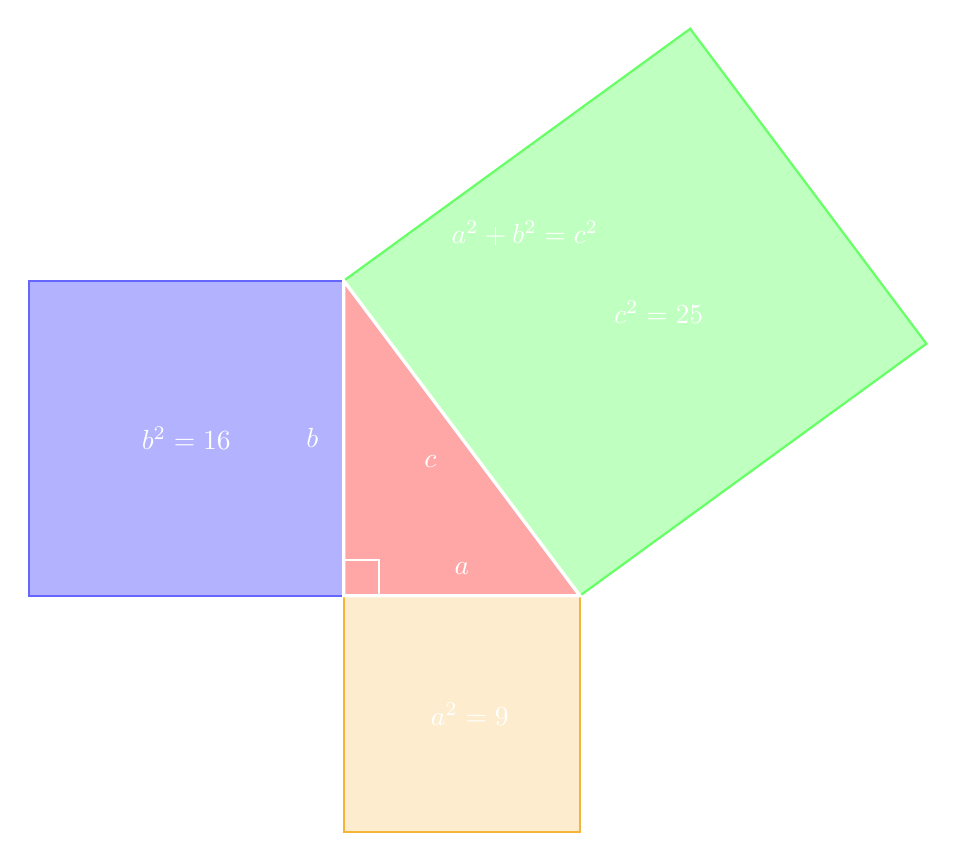
\begin{tikzpicture}[x=1cm,y=1cm,tx/.style={text=tx}]
% triangle: right angle at C(0,0), A(0,4), B(3,0)
\coordinate (C) at (0,0);
\coordinate (A) at (0,4);
\coordinate (B) at (3,0);
% square on leg a (bottom, side 3)
\fill[acc!25] (0,0) -- (3,0) -- (3,-3) -- (0,-3) -- cycle;
\draw[acc,thick] (0,0) -- (3,0) -- (3,-3) -- (0,-3) -- cycle;
% square on leg b (left, side 4)
\fill[blue!30] (0,0) -- (0,4) -- (-4,4) -- (-4,0) -- cycle;
\draw[blue!60,thick] (0,0) -- (0,4) -- (-4,4) -- (-4,0) -- cycle;
% square on hypotenuse (3-4-5)
\fill[green!25] (0,4) -- (3,0) -- (7.4,3.2) -- (4.4,7.2) -- cycle;
\draw[green!60,thick] (0,4) -- (3,0) -- (7.4,3.2) -- (4.4,7.2) -- cycle;
% triangle
\fill[red!35] (0,0) -- (3,0) -- (0,4) -- cycle;
\draw[white,very thick] (0,0) -- (3,0) -- (0,4) -- cycle;
\draw[white,thick] (0.45,0) -- (0.45,0.45) -- (0,0.45); % right angle
% labels
\node[white] at (1.6,-1.5) {$a^2 = 9$};
\node[white] at (-2,2) {$b^2 = 16$};
\node[white] at (4.0,3.6) {$c^2 = 25$};
\node[white,font=\bfseries] at (1.1,1.7) {$c$};
\node[white] at (1.5,0.35) {$a$};
\node[white] at (-0.4,2) {$b$};
\node[white] at (2.3,4.6) {$a^2 + b^2 = c^2$};
\end{tikzpicture}
\end{document}
